%% TODO:  fill in [REF]S
%% TODO:  more on FR, relate to handling time, draw pictures.
%% TODO:  sort out noise: check equations(outline.pdf and email to MG dated 12/12/14) & simulations.
 
\section{Motivation}
\label{sec:motivate_interactions}

% need to mention intra-specific interaction here?? or already mentioned in intro..
This section focuses on the interactions between species. The importance of this topic was discussed at length in the introduction (section \ref{sec:introduction}). However we re-iterate here that inter-specific interactions are one of the major mechanisms that drive ecological processes. For example trophic interactions (e.g. predator-prey) define the pathways along which energy flows through an ecological community [REF], and are responsible for both top-down and bottom-up regulation of species abundances [REF]. Similary mutualistic and competitive interactions play an important role in shaping communities [REF]. All inter-specific interactions play a role in generating the temporal pattern of species abundances that we call \emph{population dynamics}. A well known example of this is the phenomenon of predator-prey oscialltions, which are thought to have been exhibited by hare and lynx populations in Hudson Bay, Cananda [REF]. Predator-prey oscillations will play an important role in this chapter.

The modelling approach in the previous chapters was \emph{individual based}. Therefore in our simulations the interactions occured between individuals of a given species, as they do in nature. However the possibility for two individuals to interact was determined by the species interaction network - if a link between two species exists in the network then individuals belonging to those species may interact. 

....
Lacking suitable data - for which time-series and interaction (strengths) known..

Focus in predaot-rprey interactions..can be extended..

In this chapter we investiagte one novel method for inferring species interaction strengths...

Outline exactly what we will do e.g. two species focus, prey-dependenance 

\section{Methodology}
\label{sec:methods}

The general goal is to quantify inter-specific interaction strengths from observed population dynamics. As discussed, we currenlty lack suitable empircal data to do this (section \ref{sec:motivate_interactions}). Therefore we develop a methodolgy using \emph{simulated} population dynamcis. In the future this method could be applied to empircal abudnance time-series (see discussion in section \ref{sec:discussion}). The population models used for simulation are, for the most part, standard ordinary differential equation (ODE) models. These are outlined in section \ref{sec:models}. However we also present a preliminary application of our methdology to dynamics generated using the individual-based model from the previous chapters (section \ref{sec:ibm}). To quantify the interaction strengths between species from their simulated dynamics we adapt a method from \cite{shandilya2011inferring}. In short the method is used to fit a generalised Lotka-Volterra (GLV) model to the dynamics, giving numerical estimates of the interaction terms. The method is detailed in section \ref{sec:timme} and the use of the GLV model to quantify interaction strengths is justified in section \ref{sec:interaction_strength}. %% more on interaction strenght and GLV model here?


\subsection{Population models}
\label{sec:models}

%% Parameter choices. Euler method. Timestep. Extinction boundary contiditions.
%% Conventional to use N,P for predator prey, however our terminology allows easy extension to larger systems..(refer forwards to this)
%% re-order this - good choice first!

To simulate population dynamics we use coupled ordinary differential equation (ODE) models. Although we focus on dynamics generated by predator-prey interactions, the ODE modelling framework may be adapted to model other types of interaction (e.g. mutulaism, competition). ODE models have been used extensively to simulate predator-prey dynamics at the species level [REFS]. They have several limitations in their usefullness. which are discussed in \ref{sec:discussion}. However they are a suitable choice for us becuse the equations explictly contain a term that defines the interactions between species. Therefore we are able to simulate populations dynamics for which we know the analytic form of all inter-specific interactions involved. This is the key to being able to test our method for quantifying interaction strengths [SECTION?].   

We foucs on two-species systems. However the modelling framework, and the methodology in general may be extended to larger systems (see section \ref{sec:ibm}). The growth rate for each species is defined by an ODE, which takes the general form:

\begin{equation}
\frac{dx_i}{dt} = G_{i}(x_i) + \Sigma_{j=1}^{N}F_{ij}(x_i,x_j) + \xi_i,
\label{eq:general_model}
\end{equation}  

where $x_i$ is the population density of species $i$; $N$ is the number of species; $G_{i}$ is the intrinsic growth function of species $i$; $F_{ij}$ is a functional coupling between species $i$ and $j$; and $\xi_i$ is an additive noise term (see below). 

We now restrict the discussion to two species systems. However all that follows may be extended to larger systems with little modification. This possibility is discussed in section \ref{sec:discussion}\footnote{Or results presented in section...}. Writing equation \ref{eq:general_model} for both species, and expanding the coupling function $F_{ij}$ in terms of the \emph{functional response}, we can express the entire system as:

\begin{eqnarray}
\frac{dx_0}{dt} &=& G_{0}(x_0) + a_{01}x_1H(x_0,x_1) + \xi_0,  \nonumber \\
\frac{dx_1}{dt} &=& G_{1}(x_1) + a_{10}x_1H(x_0,x_1) + \xi_1
\label{eq:two_species}
\end{eqnarray}

where species 0 is the prey; species 1 is the predator; the $a_{ij}$ are constant coefficients and $H(x_0,x_1)$ is the functional reponse (FR) of the predator. The other symbols are the same as in equation \ref{eq:general_model}. The FR gives the rate at which a single predator consumes prey i.e. the per-captia predation rate. Numerous functional forms have been proposed for the FR, and as we discussed the correct form is the subject of a long running debate [REFS]. However there are some widely used forms for both the FR and the intrinsic growth function $G_i$, which we adopt. We use the following intrinsic growth functions:

\begin{eqnarray}
G_0(x_0) &=& r_0x_0\left(1-\frac{x_0}{K_c}\right)  \\
G_1(x_1) &=& -r_1x_1,
\label{eq:two_species}
\end{eqnarray}

where $r_i \in \mathbf{R}^+$ is the intrinsic growth rate of species $i$ and $K_c$ is the carrying capacity of the prey species. Therefore the predator species has an exponential intrinsic mortality, as in the Lotka-Volterra equations [REFS], whereas the prey species has a saturating growth function, as in the Rosenzweig-MacArthur model [REF]. For the FR we focus mainly on those porposed by Holling in the 1950s [REFs], which have been most widely used [REFS]. However other proposed forms of the FR are important in the debate and these are discussed in section \ref{sec:discussion}. There are three Holling FRs, types I, II, and III which can be expressed as:

\begin{eqnarray}
H_I(x_0,x_1) &=& x_0, \\
H_{II}(x_0,x_1) &=& \frac{x_0}{x_0 + K_s}, \\
H_{III}(x_0,x_1) &=& \frac{x_0^2}{x_0^2 + K_s^2},
\end{eqnarray}

where $K_s$ is the saturation constant for the predator, giving the prey density at which the per-predator consumption rate reaches half-maximum\footnote{This quantity can be related to other biologically meaningful values: search time and handling time.}. MORE ON FRS: PCITURES (OR IN SECTIONS ON IS??)

\paragraph*{Additive noise term}

Discuss what it is, why and deterministic limit. Process error [REF].
\\
We include additive noise $\xi_i$ in some simulations (see section \ref{sec:noise_explained}). Therefore the (deterministic) population dynamics of a species is entirely determined by its intrinsic growth and interaction functions.
SORT THIS OUT.

\subsection{Simulation procedure}
\label{sec:simulation_method}

\subsection{Interaction strength}
\label{sec:interaction_strength}

% emphasise that we know the interaction strength for our simulation model
% discuss other metrics here. Probably lit review?
There are numerous metrics available that can be used to quantify the strength of interactions between species. These other metrics are discussed in chapter \ref{chap:introduction} and in more detail in [REFS]. Of these metrics there is one that is a natural choice because we are able to make a direct comparison between the interaction strengths estimated from the population dynamics (using the method in section \ref{sec:timme}), and those evaluated from the simulation model (equations \ref{eq:general_model}). This metric is called the \emph{interaction matrix} (IM). The elements of the IM, $\alpha_{ij}$, quantify the effect of a small change in the population density of species $j$ on the per capita growth rate of species $i$. Therefore the IM elements are given by:

\begin{equation}
\alpha_{ij} = \frac{\partial}{\partial x_{j}}\left(\frac{1}{x_{i}} \frac{dx_i}{dt} \right),
\label{eq:IM}
\end{equation}

where $x_i$ and $x_j$ are the population densities of species $i$ and $j$ respectively. In the case of our two species systems the IM is a $2 \times 2$ matrix, but trivially extends to quantify all pair-wise interactions between species in a $N$-species system. Since our simulation model has an explicit form for $\frac{dx_0}{dt}$ and $\frac{dx_1}{dt}$ we can evaluate the parital derivative in equation \ref{eq:IM} to obtain analytic forms for all the IM elements ($\alpha_{00}$, $\alpha_{01}$, $\alpha_{10}$,$\alpha_{11}$). That is, we can calculate the interaction strengths exactly from our simulation model. 


However, as stated, our goal is quantify the interaction strengths using only the population dynamics. In order to do this we fit an ODE modle to the  

\subsection{Inference method}
\label{sec:timme}

%% Dealing with extinctions. Range sampling - diagrams!!

\subsection{Examples}
\label{sec:method_examples}

%% include here an example of both Linear and HII dynamics (with mean interaction strength), and to demonstrate noise levels. And the results that we get from tinference. And an examples of range samplig (refer forwards to dsicusssion) 

\begin{figure}[h]
\centering 
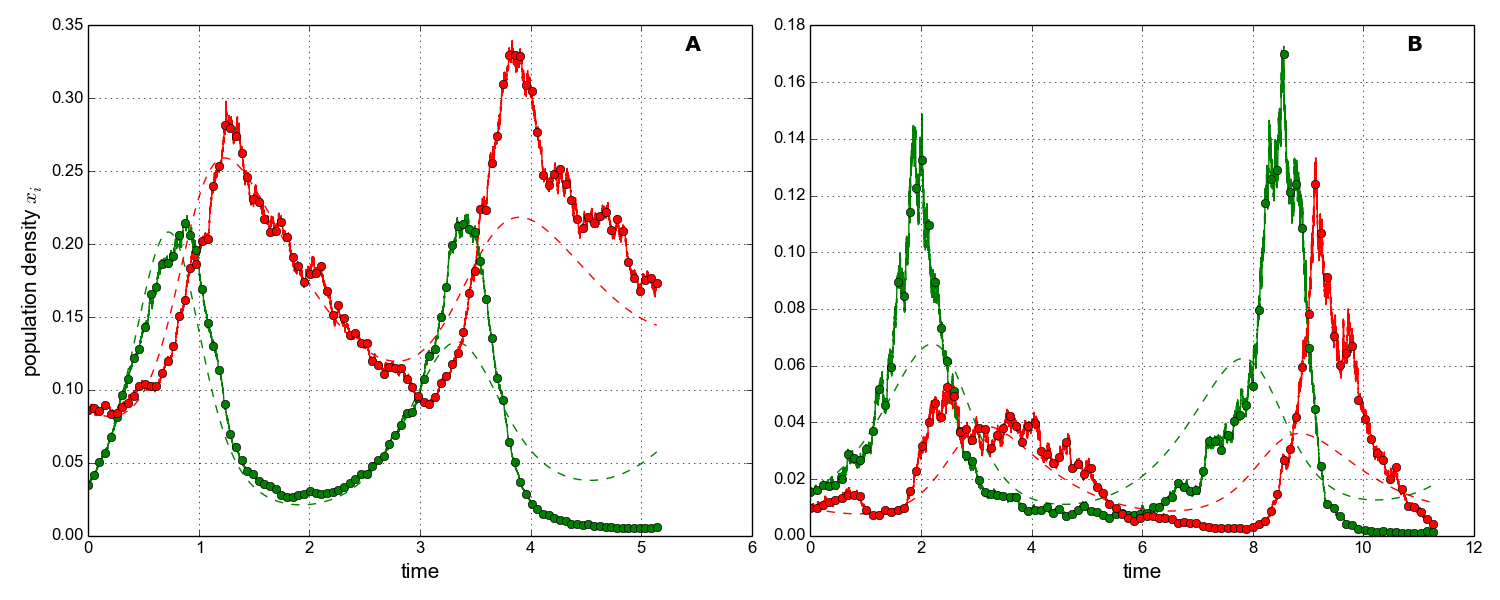
\includegraphics[width=\textwidth]{{{figures/example_dynamics_pID_0_and_87_noise_20.000000}}}
\caption{Example linear dynamics. 100 sampels. Two different parameter sets. A: noise=20. B:noise=50.} 
\label{fig:ex_dynamics_linear}
\end{figure}

\begin{figure}[h]
\centering 
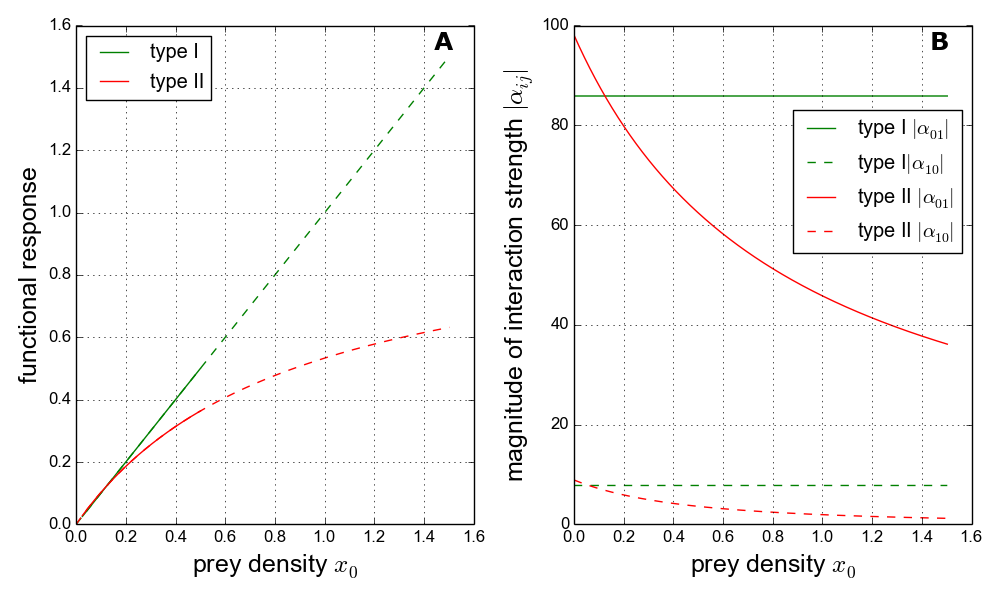
\includegraphics[width=0.8\textwidth]{{{figures/FR_example}}}
\caption{Example FR. Parameters?} 
\label{fig:fr_example}
\end{figure}


\clearpage
%\afterpage{%
\thispagestyle{empty}
\begin{sidewaysfigure}

		\centering      
		\hspace{-3cm}

        %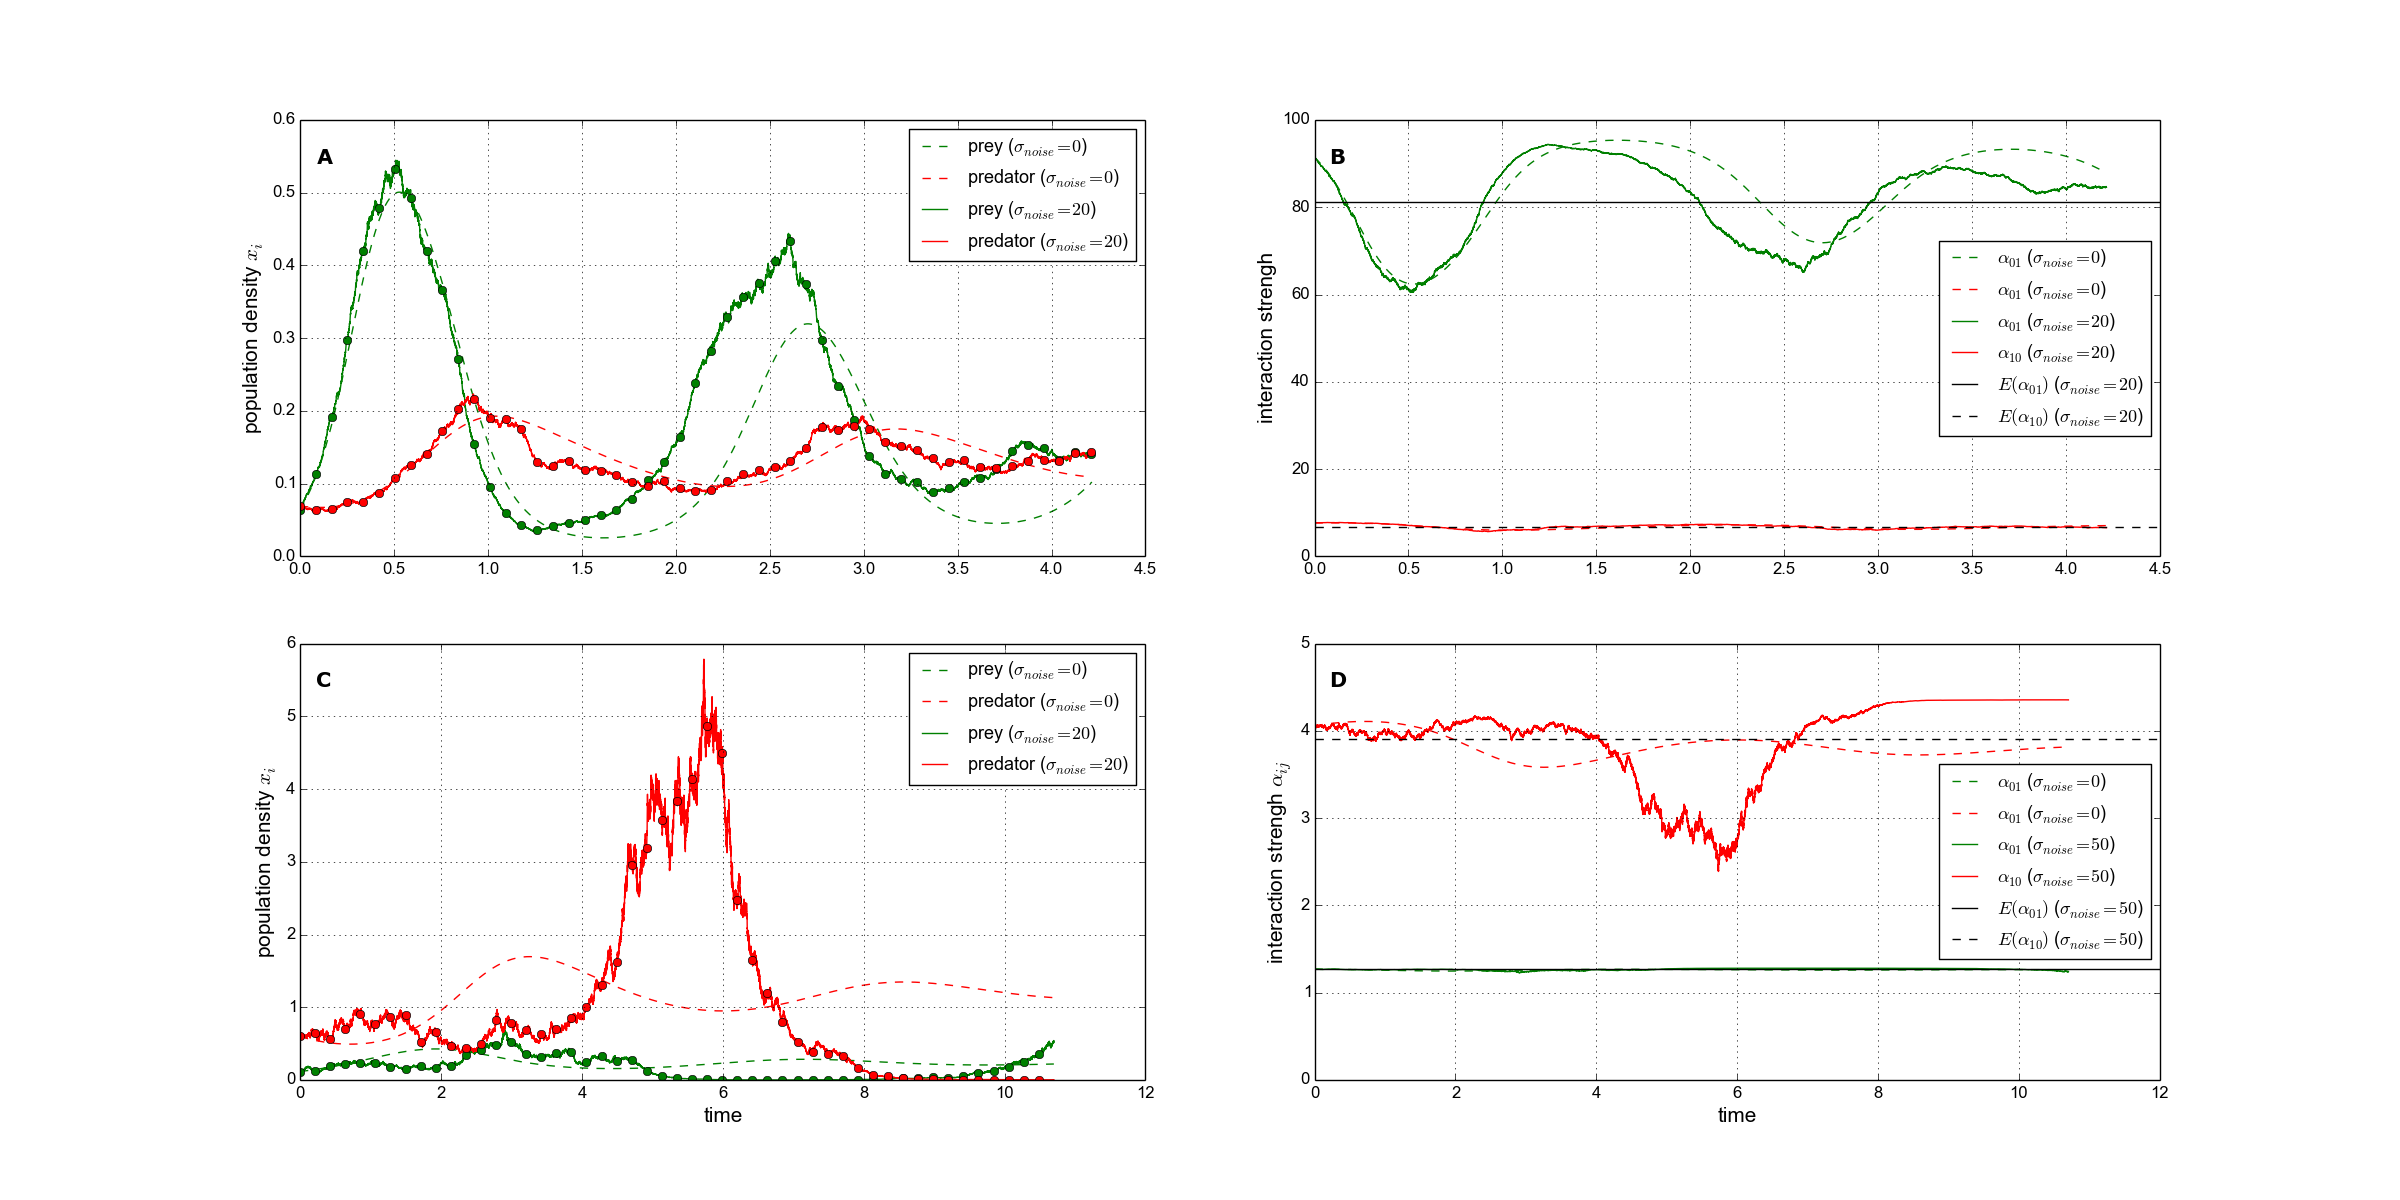
\includegraphics[width=\linewidth]{{{figures/example_dynamics_HII_pID_7_and_0}}}
		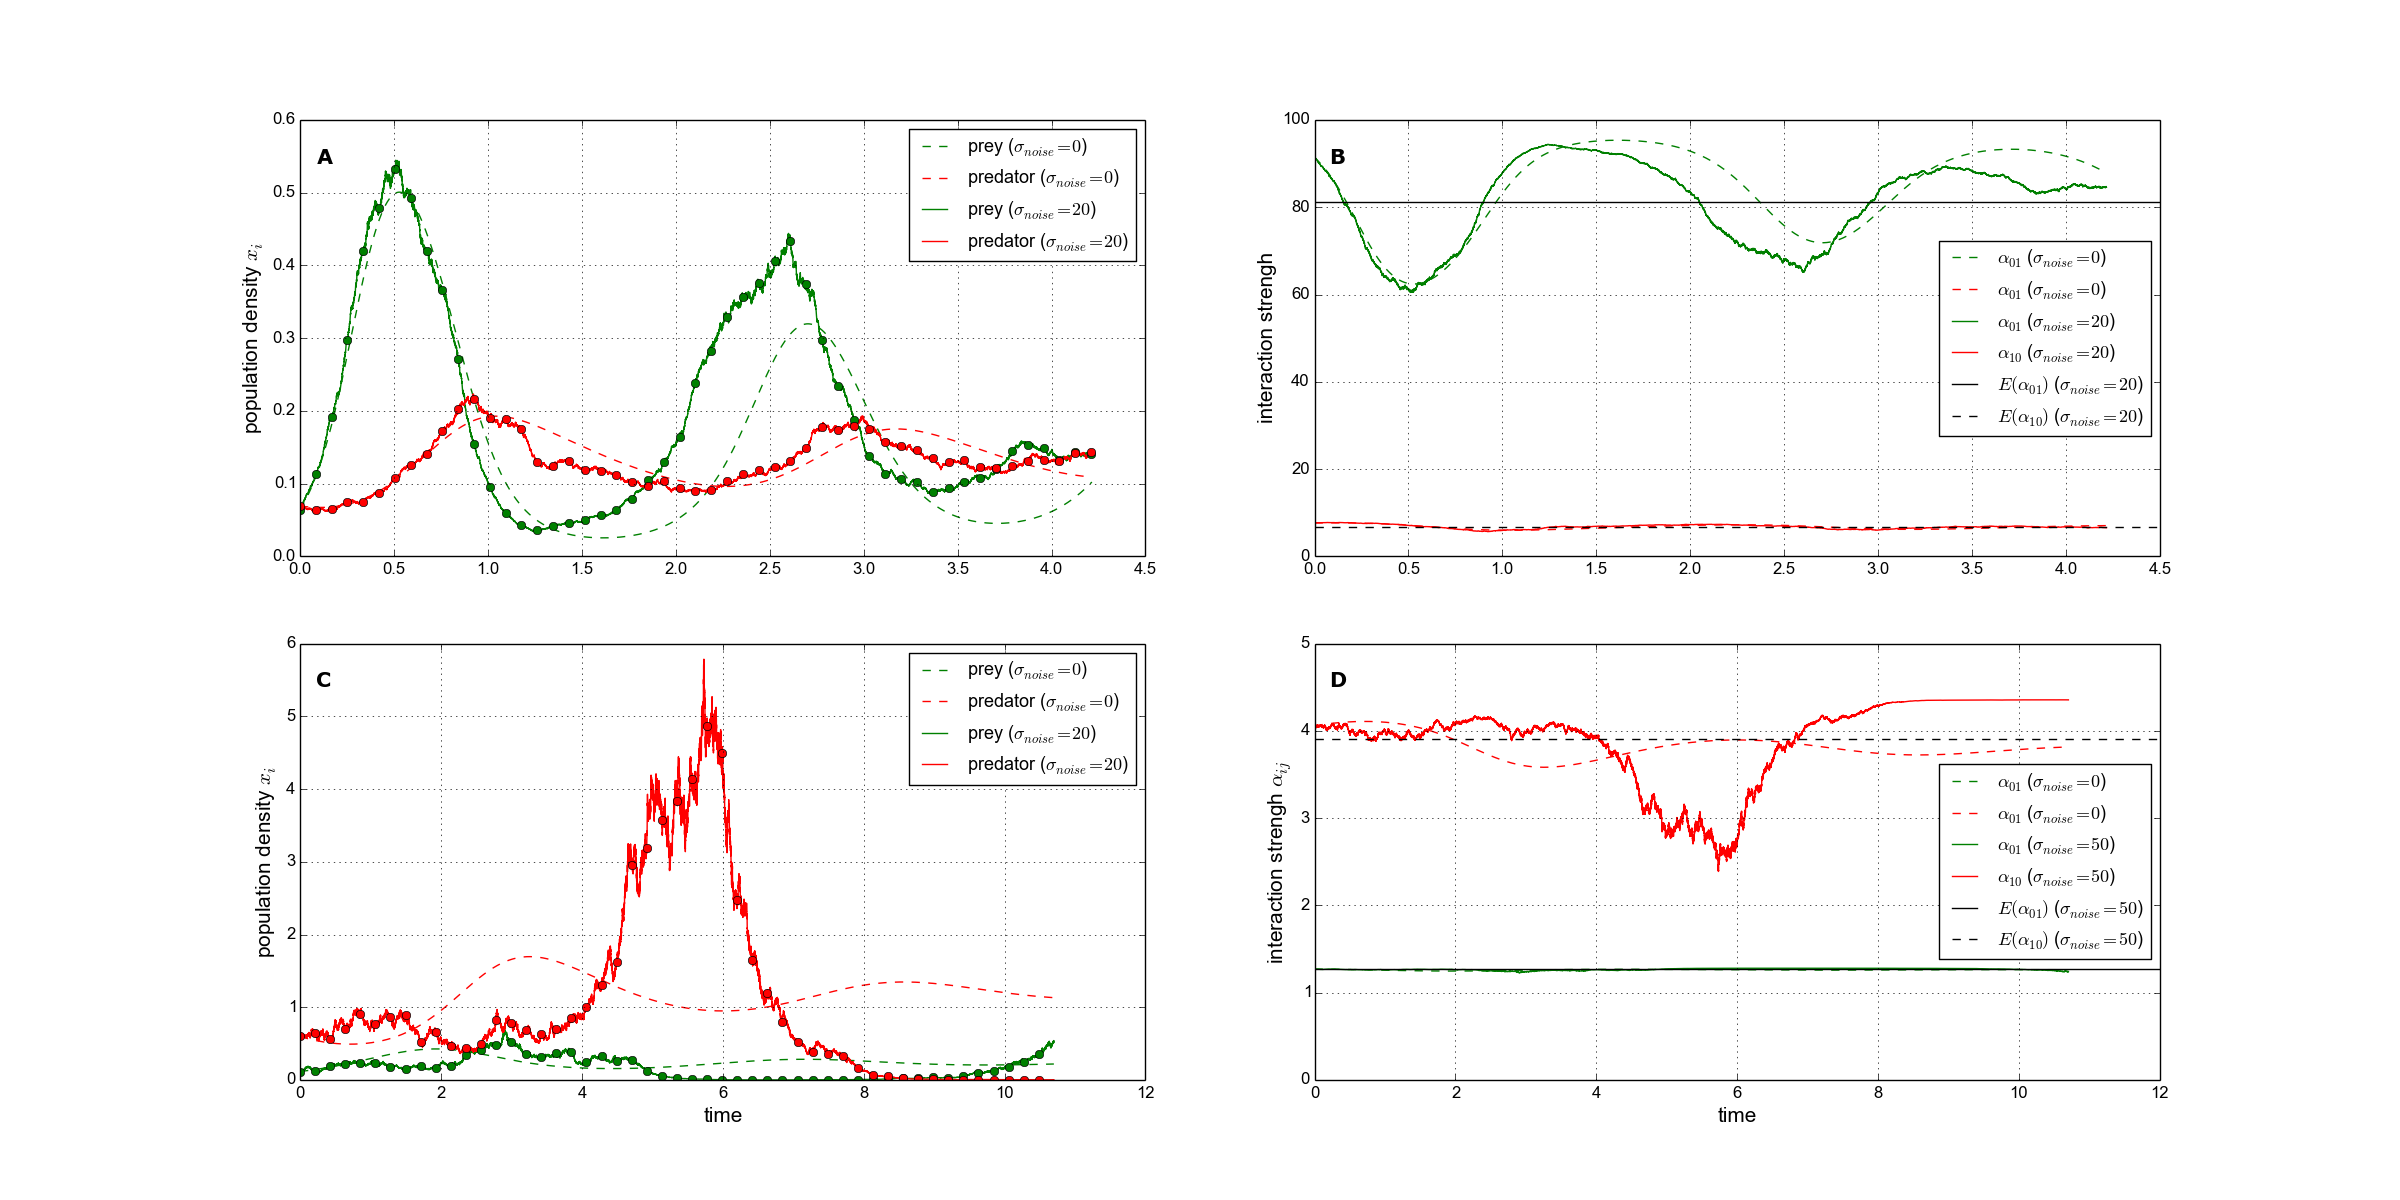
\includegraphics[width=\textwidth]{{{figures/example_dynamics_HII_pID_7_and_0}}}
        \caption{Example HOlling II dynamics.}\label{fig:ex_dynamics_holling}
        %% Note: this figure generated by Documents/IM_vs_HL_heatmap/plot_sum_maps.py
\end{sidewaysfigure}
\clearpage
%}

\section{Results}
\label{sec:results}

% some of this description goes above - for example some need explaining before previous section(examples)
In this sections we characterise the numerical performance of the method, described in section \ref{sec:timme}, for estimating the strength of interactions between species. The method is tested on the dynamics of two different ODE systems: a Lotka-Volterra (LV) and a Holling type II (HII) system. In the first case it is simply a test of a model fitting procedure. This is because the method works by fitting a generalised Lotka-Volterra (GLV) model to the dynamics, and he LV systems can be expressed as a GLV systems. Therefore we are simply simulating using one model, and then testing a method of estimating the model parameters form the simulated dynamics. We test the effects of noise and sampling frequency. In the second case, the HII system cannot be expressed as a GLV system. Therefore the GLV model that we fit can only approximate the dynamics and we cannot make a direct comparison between the parameters of the simulation model and the GLV model used for estimation. In this case we comapre to the mean interaction strengths (see section \ref{sec:res_hii}.


\subsection{Lotka-Volterra system}
\label{sec:res_glv}

Initially we run repeated simulations of the LV model using a single parameter set. We investigate how the numerical estimates of the model parameters respond to two variables: the level of noise in the simulations; and the number of samples used for estimation. Other variables are held constant using the simulation procedure described in section \ref{sec:simulation_method}. We then generalise these results by looking at the relative error in the estimates, for repeated simulations using an ensemble of 100 selected parameter sets (as described in section \ref{sec:simulation_method}).

\paragraph*{Single parameter set.}

Here we can make direct comparison between model parameters. The GLV model for two species has six parameters: $r_0,r_1,J_{00},J_{01},J_{10},J_{11}$. These correspond respectively to the following constant values of the LV system used for simulations: $A,-1,-A,-B,C,0$ (see equation \ref{eq:WHEREIS}). In general we find that the numerical estimates perform well at low noise intensities and poorly at high noise intensities. This is illustrated in figures \ref{fig:sp_v_n_100} and \ref{fig:sp_v_n_10000}. We also find that the estimates improve with the number of samples used, up to a point. Beyond this point the use of more samples does little to improve to estimates, and in some cases makes them worse. This behaviour is illustrated in figures \ref{fig:sp_v_ns_10} and \ref{fig:sp_v_ns_50}. These patterns were found to hold across all parameter sets investiagted, but are only shown using a single parameter set here for clarity.

In panel \textbf{A} of figures \ref{fig:sp_v_n_100} and \ref{fig:sp_v_n_10000} we see that the mean value of the estimates approaches the true value for low noise and, in panel \textbf{B} that the variance in the estimates approaches zero. This tells us that the method consistently gives a good fit of the GLV to the dynamics of the LV system, even when only 100 sample points are used (figure \ref{fig:sp_v_n_100}). As the noise intesitiy is increased the mean values of the estimates deviate from the true values, and the standard deviation in the estimates increases. Comparing the two figures we see that the response to noise is very similar whether 100 or 10,000 samples are used. A notable exception to this is a spike in the variance in panel \textbf{B} of figure. However this appears to be a single statistically anomolous result and not part of the trend. Panel \textbf{C} of both figures shows that the error function, which is minimised by the estimation method, increases with noise for both species. This cannot be directly compared between the two plots because of the different number of samples used. However it indicates that in both cases (100 and 10,000 samples) the quality of the fit is high in the deterministic case, and decreases with noise. 

\begin{figure}[h]
\centering 
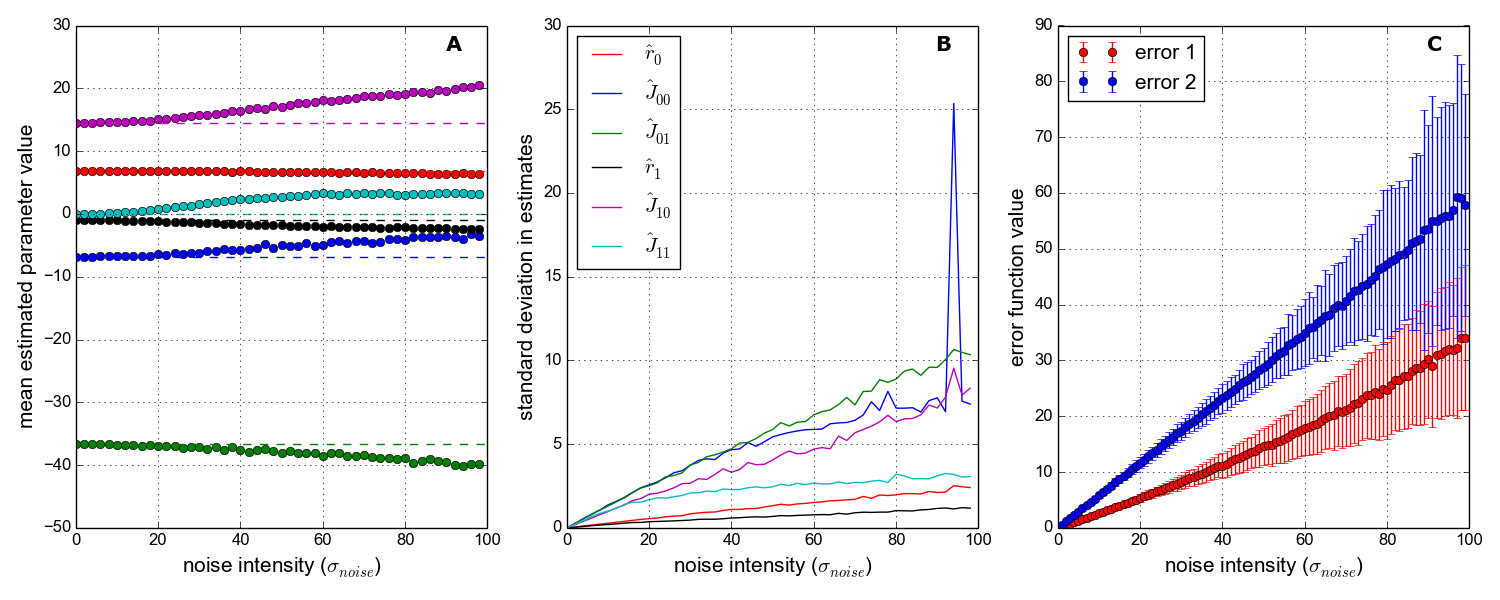
\includegraphics[width=\textwidth]{{{figures/single_params_v_noise_pID_0_nsamples_100}}}
\caption{Effect of noise on numerical estimates. Here the method uses 100 samples from simulated dynamics. All simulations run using the LV model with a single parameter set. The noise intensity varies between 0 (deterministic) and 100. See section \ref{sec:method_examples} for an intuition of how noisy this is. 1000 repeat smulations run at each noise level. \textbf{Panel A}: Mean estimated parameter values (each dot representing mean over 1000 repeats). The `true' paramter values of the simulation model are shown by dashed lines. \textbf{Panel B:} Standard deviation in estimates. \textbf{Panel C:} Value of the error functions used in the estimation method, one for each species. The dots show the mean error, and the bars show $\pm$ one standard deviation.}
\label{fig:sp_v_n_100}
\end{figure}

\begin{figure}[h]
\centering 
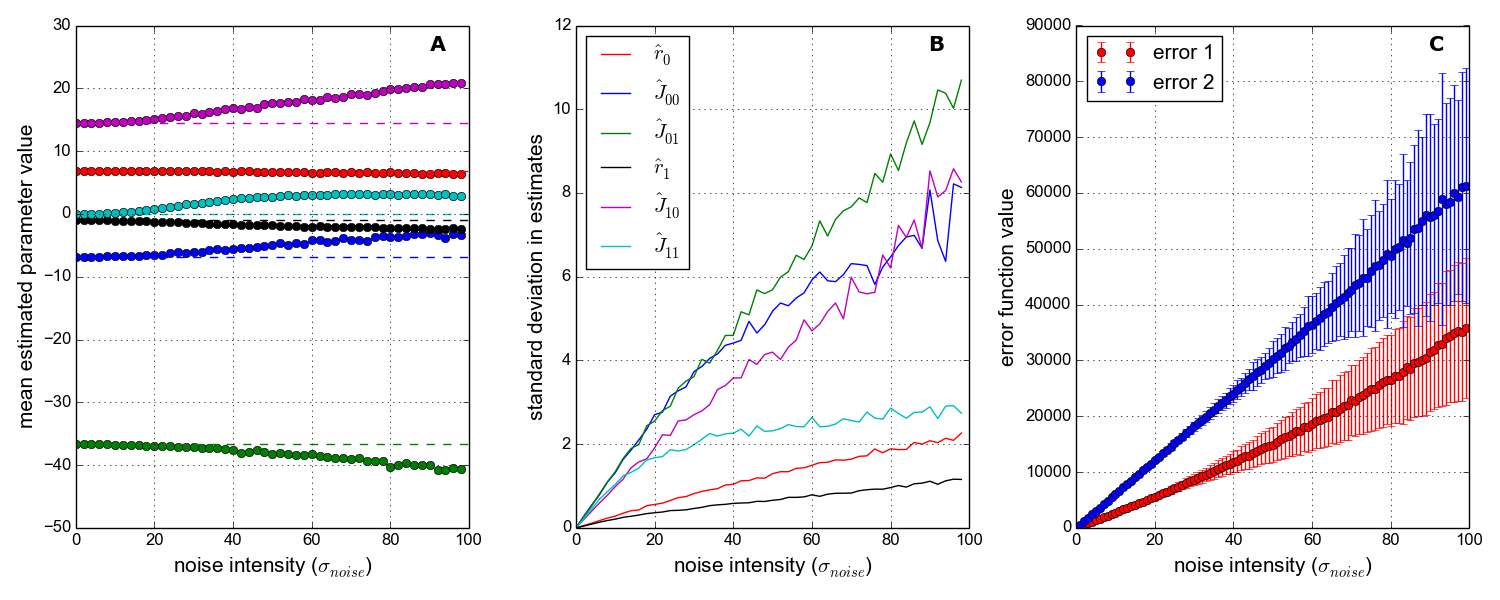
\includegraphics[width=\textwidth]{{{figures/single_params_v_noise_pID_0_nsamples_10000}}}
\caption{Exactly as in figure \ref{fig:sp_v_n_100} but using 10,000 samples from the simulated dynamics.} 
\label{fig:sp_v_n_10000}
\end{figure}

We now look at how the estimates respond to the number of samples used, in the cases of low and high noise intensity. Figure \ref{fig:sp_v_ns_10} shows the low noise case, with $\sigma_{noise}=10$. In panel \textbf{A} we see that the mean value of the estimates quickly converges to close to the true parameter values, as the number of samples increases. Panel \textbf{B} shows that the standard deviation in the estimates quickly becomes small, but non-zero. Above about 32 samples there is no visible improvement in the estimates, as measured by the mean or standard deviation. In figure \ref{fig:sp_v_ns_50} we see the effect of a higher noise intensity. Here we have $\sigma_{noise}=50$. Panel \textbf{A} shows that the estimates do not converge on the true parameter values, even for large numbers of samples. Also the standard deviation in the estimates, shown in panel \textbf{B}, is higher than in the low noise case. Again we find that there is little, if any, improvement in the estimates beyond about 32 samples. 
%% also general ruel: intirnsic growth parameters are better matched..

\begin{figure}[h]
\centering 
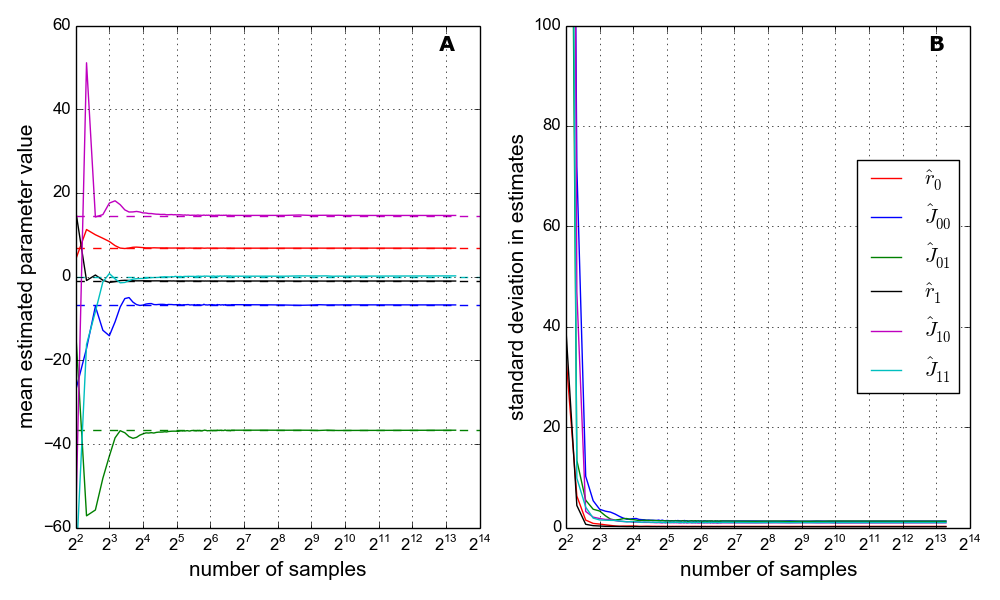
\includegraphics[width=0.67\textwidth]{{{figures/single_params_v_nsamples_pID_0_noise_10.000000}}}
\caption{Effect of the number of samples on numerical estimates. All simulations run using the LV model with a single parameter set. The noise intensity $\sigma_{noise}=10$. Number of samples ranges from 4 to 10,000. Samples drawn from  simulated dynamics at equal intervals. 1000 repeat smulations for each number of samples. \textbf{Panel A}: Solid lines show mean estimated parameter values. Dashed lines show the `true' paramter values of the simulation model. \textbf{Panel B:} Standard deviation in estimates.}
\label{fig:sp_v_ns_10}
\end{figure}

\begin{figure}[h]
\centering 
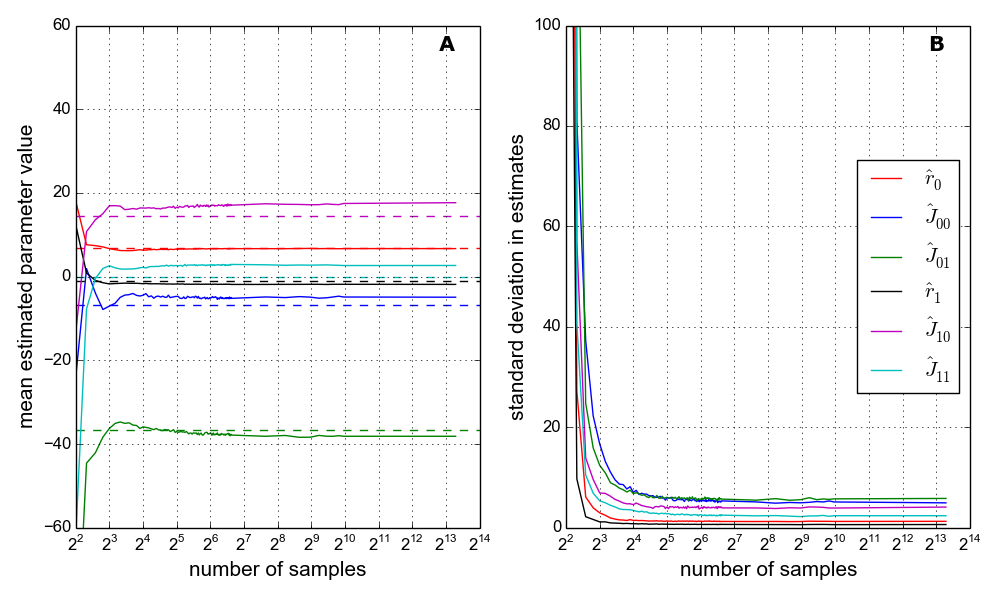
\includegraphics[width=0.67\textwidth]{{{figures/single_params_v_nsamples_pID_0_noise_50.000000}}}
\caption{Exactly as in figure \ref{fig:sp_v_ns_10} but with noise intesity $\sigma_{noise}=50$.} 
\label{fig:sp_v_ns_50}
\end{figure}

\paragraph*{Ensemble of parameter sets.}

Run 10 repeats for each of 100 parameter sets. In general the trends described above hold across the ensemble..

\begin{figure}[h]
\centering 
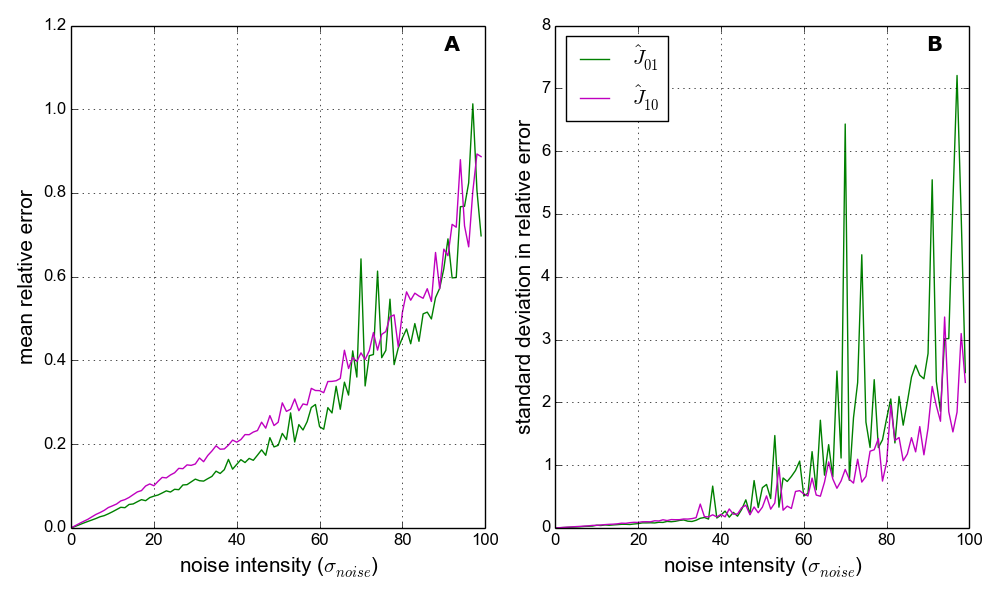
\includegraphics[width=0.67\textwidth]{{{figures/ensemble_params_vs_noise_nsamples_1000}}}
\caption{Nonsense. 1000 samples used.} 
\label{fig:ep_v_n}
\end{figure}

\begin{figure}[h]
\centering 
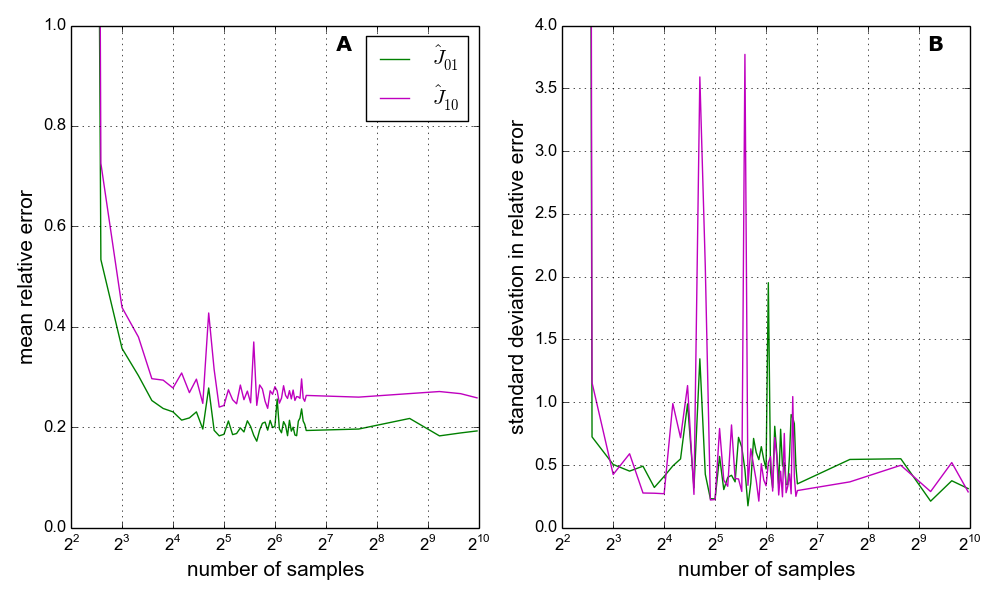
\includegraphics[width=0.67\textwidth]{{{figures/ensemble_params_vs_nsamples_noise_50.000000.IS}}}
\caption{Nonsense. Noise is 50.} 
\label{fig:ep_v_ns}
\end{figure}




\subsection{Holling system}
\label{sec:res_hii}

\begin{figure}[h]
\centering 
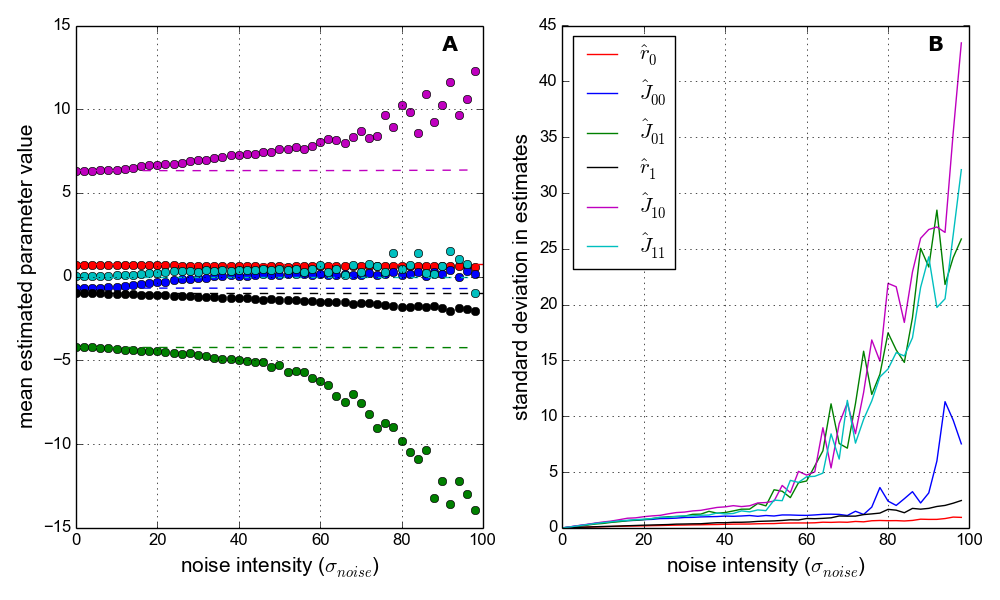
\includegraphics[width=0.67\textwidth]{{{figures/single_params_v_noise_pID_87_nsamples_10000.HII}}}
\caption{Nsamples is 10,000.} 
\label{fig:hii_sp_v_n}
\end{figure}

\begin{figure}[h]
\centering 
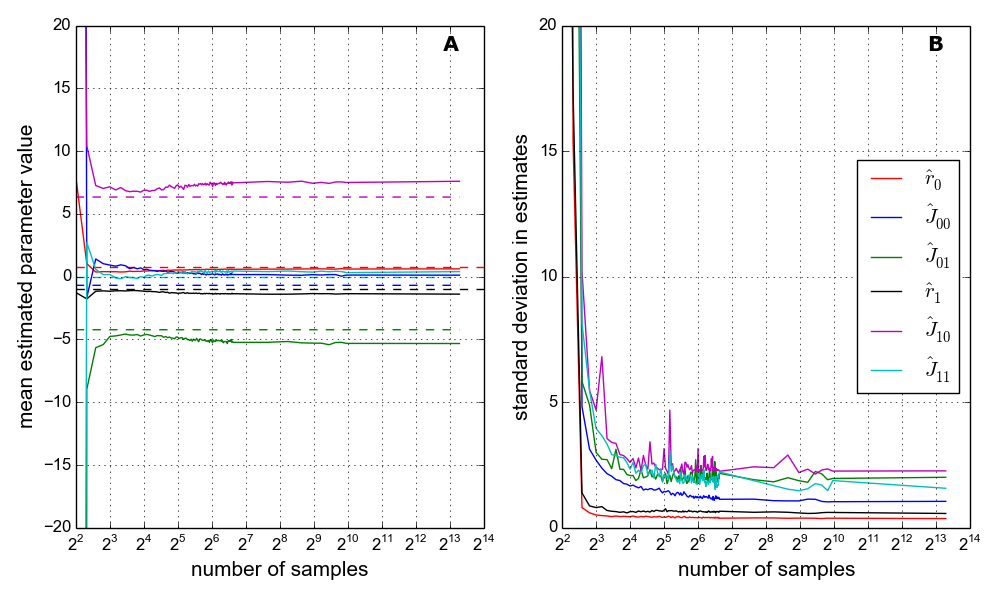
\includegraphics[width=0.67\textwidth]{{{figures/single_params_v_nsamples_pID_87_noise_50.000000.HII}}}
\caption{Noise is 50.} 
\label{fig:hii_sp_v_ns}
\end{figure}

\begin{figure}[h]
\centering 
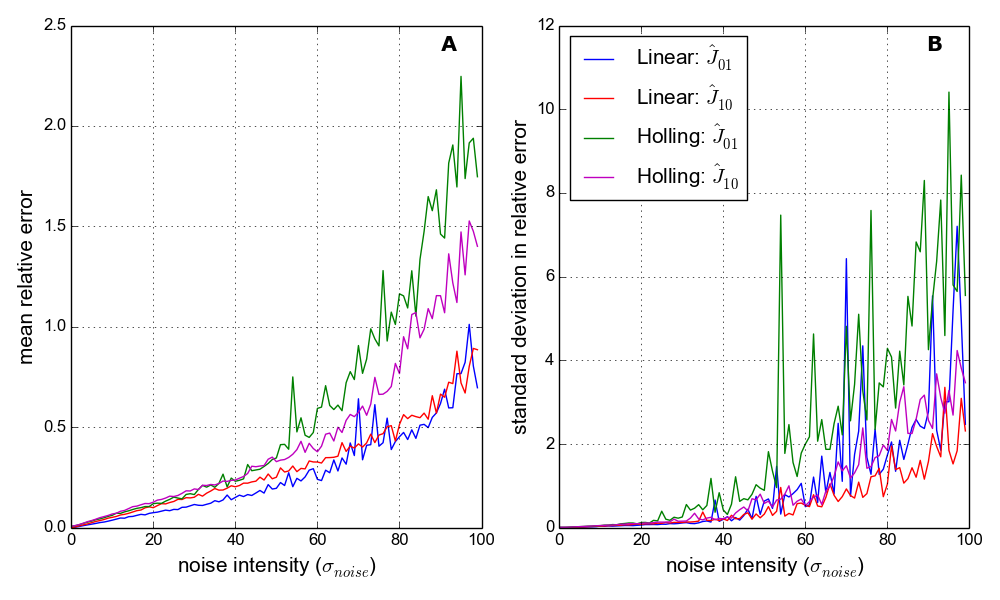
\includegraphics[width=0.67\textwidth]{{{figures/ensemble_params_vs_noise_nsamples_1000.B}}}
\caption{Noise is 50.} 
\label{fig:hii_ep_v_ns}
\end{figure}

\begin{figure}[h]
\centering 
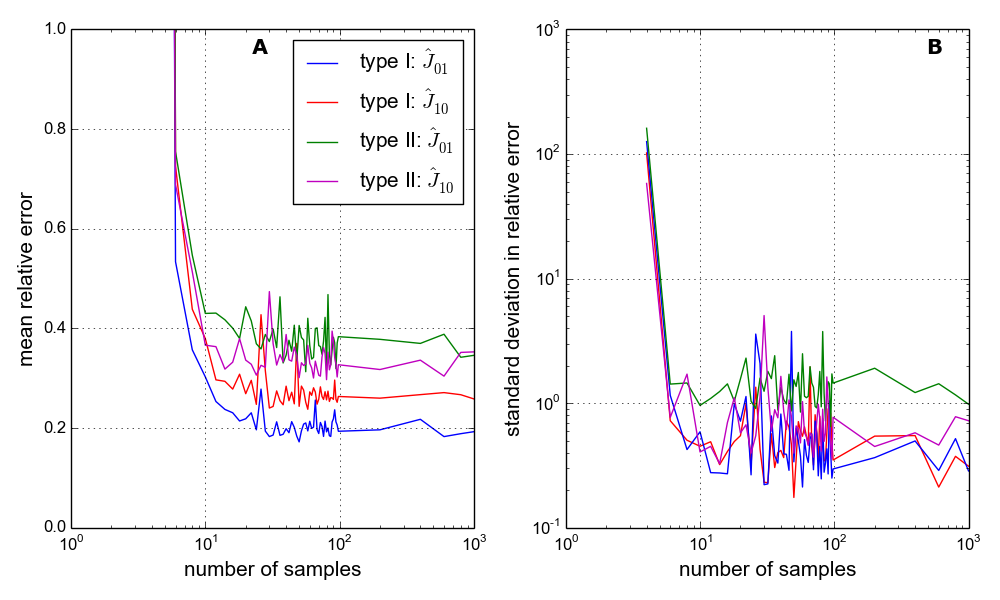
\includegraphics[width=0.67\textwidth]{{{figures/ensemble_params_vs_nsamples_noise_50.000000.B.IS}}}
\caption{Noise is 50.} 
\label{fig:hii_ep_v_ns}
\end{figure}


\subsection{Range sampling}
\label{sec:res_range_sampling}

%% Discussion of these results first??

% > only very few samples needed really!

\section{TEMP : other results}

This section shows some plots which I was not planning to put into the thesis but are worth discussing..

\begin{figure}[h]
\centering 
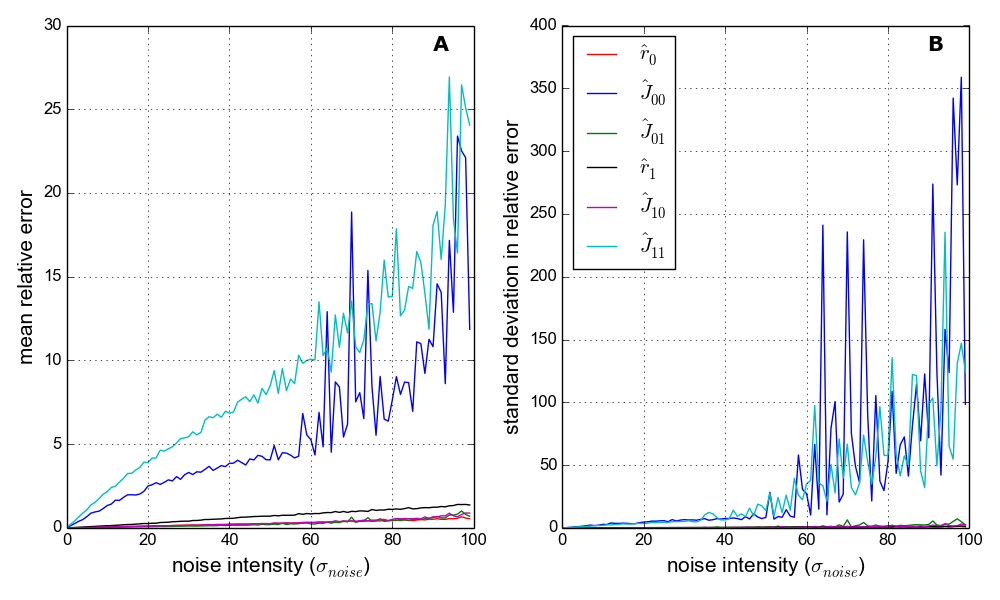
\includegraphics[width=0.67\textwidth]{{{figures/ensemble_params_vs_noise_nsamples_1000.ALL}}}
\caption{Nonsense. 1000 samples used.} 
\label{fig:ep_v_n}
\end{figure}

\begin{figure}[h]
\centering 
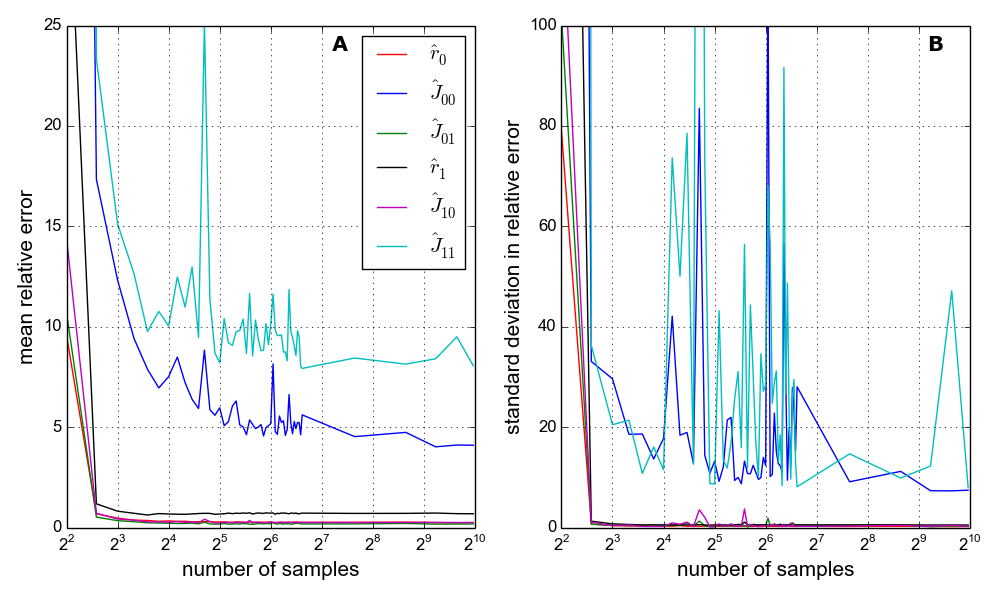
\includegraphics[width=0.67\textwidth]{{{figures/ensemble_params_vs_nsamples_noise_50.000000.ALL}}}
\caption{Nonsense. Noise is 50.} 
\label{fig:ep_v_ns}
\end{figure}

\section{Application to IBM (optional)}
\label{sec:ibm}

\subsection{Testing functionl response}
\subsection{Extend methodology (3 and 4 species)}
\subsection{Results}

%% TOD DISCUSS RE IBM APPLICATION:

% > could introduce non-linearities to IS. E.g. hanlding time?
% > discuss application to larger system. Functional groupings...etc.
\section{Discussion}
\label{sec:discussion}

Points referenced in text above, make sure to discuss them!..

\begin{itemize}
	\item Discuss how this methodology could be used on empircal data...
	\item Limitations of ODE models (non-spatial, repsonse to debate on FR)
	\item Possibility of extending to more than two specie systems (if this is actually done then change ref in text above)
	\item discussion of other forms of FR (not H) - or disucssed already in inro?
	
	\item good GLV fit to LV even with 100 sample points - realistic?
\end{itemize}
